\documentclass[11pt,a4paper]{article}
\usepackage[francais]{babel}%
\usepackage[T1]{fontenc}% 
\usepackage[utf8x]{inputenc}
\usepackage{amsmath}
\usepackage{graphicx}
\usepackage{hyperref}
\usepackage{setspace}
\usepackage{tabularx}

\renewcommand\thesection{\arabic{section}}
\begin{document}
\linespread{0.99}
\hyphenpenalty=750

\date{05 Septembre 2016}
\newcommand{\mydate}{\formatdate{4}{7}{2016}}

\begin{titlepage}
\newcommand{\HRule}{\rule{\linewidth}{0.5mm}}
\centering

\textsc{\large \textbf{Université Paris Ouest Nanterre La Défense}}\\[1.5cm] % Name of your university/college

% * <lhillah@u-paris10.fr> 2016-08-17T09:04:55.535Z:
%
% > 
\includegraphics[]{upond.PNG}\\
%
% Logo doit être moins plus discret dans le placement, pas en plein milieu.
%
% ^.
\textsc{\large Rapport d'activité de Master 2 MIAGE}\\[0.5cm] % Major heading such as course name
\textsc{\large Département Mathématiques et Informatique}\\[0.5cm] % Major heading such as course name
\textsc{\large UFR SEGMI}\\[0.5cm] 
\HRule \\[0.4cm]
{ \large  \textbf{Credit Management}:\\ Appui au pilote risque de credit au sein du Groupe EDF dans le marché d'affaires }\\[0.4cm] % Title of your document
\HRule \\[1cm]
\emph{Soutenu par \textbf{Moussa KANOUTE}}\\ le 05/09/2016\date{04 Juillet 2016}\\[1cm]
\large En vue de l'obtention du grade de Master de l'université Paris Ouest Nanterre La Défense
\\[1cm]
\begin{minipage}{0.4\textwidth}
\begin{flushleft} \large
\emph{Responsable de la filière Miage par voie classique:} \\
Pr \textbf{Pascal Poizat} % Supervisor's Name

\end{flushleft}
\end{minipage}
~
\begin{minipage}{0.4\textwidth}
\begin{flushright} \large
\emph{Tuteur enseignant:}\\
Dr \textbf{Lom HILLAH}\\
\emph{Tuteur entreprise:}\\
M \textbf{Eric STOLL}, Pilote risque de crédit chez EDF
\end{flushright}
\end{minipage}\\[2cm]
\date{05 Septembre 2016}

\vfill

\includegraphics[width=3cm]{upond.PNG} 
\hfill 

\includegraphics[width=3cm]{logo_edf_carre.png} 
\end{titlepage}

~
\thispagestyle{empty}
\newpage


\newpage
\section*{Remerciements}
\thispagestyle{empty}
Avant d’entamer la présentation de ce travail, je voudrais d’abord adresser mes sincères remerciements et reconnaissances à tous ceux qui m’ont, si efficacement, aidé à effectuer
mon alternance dans de bonnes conditions.\\

En particulier, à mon tuteur en entreprise, Monsieur Eric STOLL, souhaitant qu’il trouve ici l’expression de ma profonde reconnaissance pour sa disponibilité, ses critiques et ses précieux conseils qu’il m’a accordé tout au long de ce travail.
Mes remerciements vont également à tous les membres de l’équipe Credit Management.\\

Je souhaite aussi remercier mon Tuteur enseignant, Monsieur Lom HILLAH pour ses precieux conseils et son assistance. Je   remercie également l’ensemble de l’équipe pédagogique qui nous a suivi tout au long de cette dernière année de master MIAGE.\\

Enfin, j'adresse mes remerciements à mes parents pour leurs sacrifices, leurs confiances et tout le soutien qu'ils m'ont accordé tout au long  de mes études. \\


\newpage
\setcounter{page}{1}
\section*{Introduction}



\tableofcontents
\thispagestyle{empty}
\newpage
\listoffigures

\newpage
\section{Présentation du groupe EDF \label{presentation_groupe}}
Premier électricien mondial, le groupe EDF rassemble tous les métiers de la production, du commerce et des réseaux d’électricité.\\\\

En s’appuyant sur l’expertise de ses équipes, sa récherche et développement et son ingénierie, son expérience d’exploitant industriel et l’accompagnement attentif de ses clients, EDF apporte des solutions compétitives qui concilient développement économique et préservation du climat \cite{edf}.\\
L’enjeu pour EDF reste aujourd’hui de produire l’énergie la plus propre possible. Deux obstacles majeurs sont aujourd’hui à surmonter: la demande de plus en forte et la nécessité d’avoir une production de plus en plus propre. EDF a donc désormais un triptyque de contraintes à savoir: une énergie sûre, décarbonée et abordable. 

EDF est présent sur toutes les activités du système électrique : production, transport, distribution, commercialisation; et est présent dans une grande partie du monde. Au total, le groupe EDF produit 623,5 TéraWatt-heures (TWh) soit 623 500 000 000 Kilowatt-heures. Cela correspond à la consommation de plus de 92 millions de français (moyenne de consommation par français / an: 6 762 KWh). 

L’équilibre de son mix énergétique (nucléaire, thermique, hydraulique, énergies nouvelles) permet de répartir les risques et de faire face aux aléas du coût des énergies primaires. La figure \ref{figure_production} montre la répartion énergetique du groupe.  

\begin{figure}
 \centering
 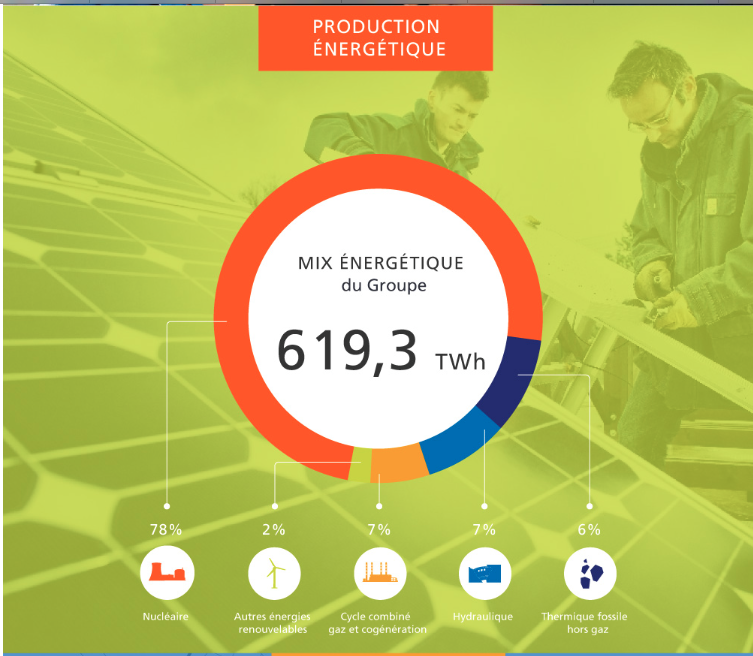
\includegraphics[scale=0.5]{production.png}
 \caption{Répartition de la production énergetique à EDF (Source: EDF)}
 \label{figure_production}
\end{figure}
Aujourd’hui EDF est le premier producteur d’énergies nouvelles et renouvelables en Europe grâce à ses 12 milliards d’euros d’investissements dans les énergies hydrauliques, solaires, éolien et maritimes.
Le groupe est également le premier réseau électrique d’Europe et premier exploitant nucléaire mondial.
Cette situation lui permet d’atteindre un Chiffre d’Affaires (CA) de 72,9 milliards d’euros.

\subsection{Organisation du groupe}
La machine EDF nécessite des ressources humaines importantes pour pouvoir assurer sa qualité de service, la sécurité de son activité industrielle et le management des ressources internes. 158161 salariés. Une telle concaténation de compétences nécessite une organisation structurée.\\
Dans ce rapport d’activité, je ne présenterai qu’une partie de l’organigramme managérial D’EDF SA, hors filiales. Chaque société dispose de ses propres directions en fonction de l’activité et de ses propres services.

\subsection{La direction commerce}
La Direction Commerce gère plus précisément l’activité «Revente» de l’énergie. Elle assure à EDF la conservation de ses parts de marché et développe le portefeuille de clients professionnels, institutionnels et particuliers. La direction est organisée en deux parties: les Directions Régionales et la Direction Nationale.\\
La Direction Commerce Nationale, se charge plus particulièrement du support pour les commerciaux en région, mais également coordonne certaines actions pour l’ensemble des clients sur le territoire. \\
La Direction marchés entreprises et professionnels, coordonne plus précisément les entreprises clientes d’EDF, des grands-comptes (importantes sociétés industrielles) jusqu’aux Très Petites Entreprises (Le médecin de quartier, le boulanger, …).\\ 
Le service Pilotage Expertise ProjetS (PEPS), manage les outils opérationnels liées aux activités de vente de la création de l’offre commerciale jusqu’aux procédures de vente. La figure \ref{figure_organigramme} montre l'organigramme de la direction commerce du groupe. 

\begin{figure}[h]
 \centering
 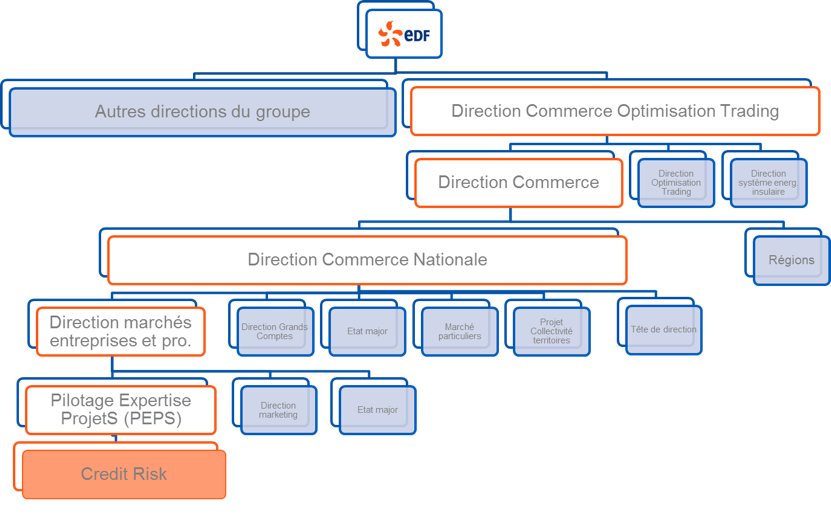
\includegraphics[scale=1.2]{direction_commerce.png}
 \caption{Organigramme de la direction commerce EDF}
 \label{figure_organigramme}
\end{figure}

\section{Le service Credit Risk ou Credit Management}
\subsection{Les missions du Credit Management}
Le service Credit Management à plusieurs missions destinées à optimiser le Besoin en Fond de Roulement (BFR). 
Il est composé d’un responsable de département, de six Credit Managers Seniors, d’une personne en charge du pilotage du Credit Management, une personne en charge du pilotage du recouvrement. 
De plus, deux membres de l'équipe sont détachés partiellement en tant que juge auprès du Tribunal de Commerce de Paris et apportent leurs expertises pour les procédures de recouvrements judiciaires des créances impayées. A l’équipe permanente s’ajoute quatre jeunes en alternance. 
Le service n’est pas centralisé en un lieu de travail. 
La plus grande partie de l’équipe est localisée à Courbevoie, dans le quartier d’affaires de La Défense. Certains membres de l’équipe sont à Nantes, Lille, Nancy et Lyon.
Pour pallier à cet éloignement géographique, des réunions entre analyses sont organisées de façon régulière pour échanger sur les pratiques «métier» et la vie de l’équipe. L’ensemble des membres de l’équipe ont accès à une base d’information commune reprenant les éléments de la procédure de scoring, des fiches d’information, des outils de formation et des espaces à diffusion restreinte.
Du fait de ses missions, le service n’est jamais en contact direct avec les clients d’EDF. La grande majorité des échanges sont internes, vers les commerciaux et certains gestionnaires. Les missions du service de Credit Management sont confidentielles, ainsi que les sources d’informations, les méthodes de scoring et les données transmises par les clients. La figure \ref{figure_cm} montre la composition du service Credit Management
\begin{figure}[h]
 \centering
 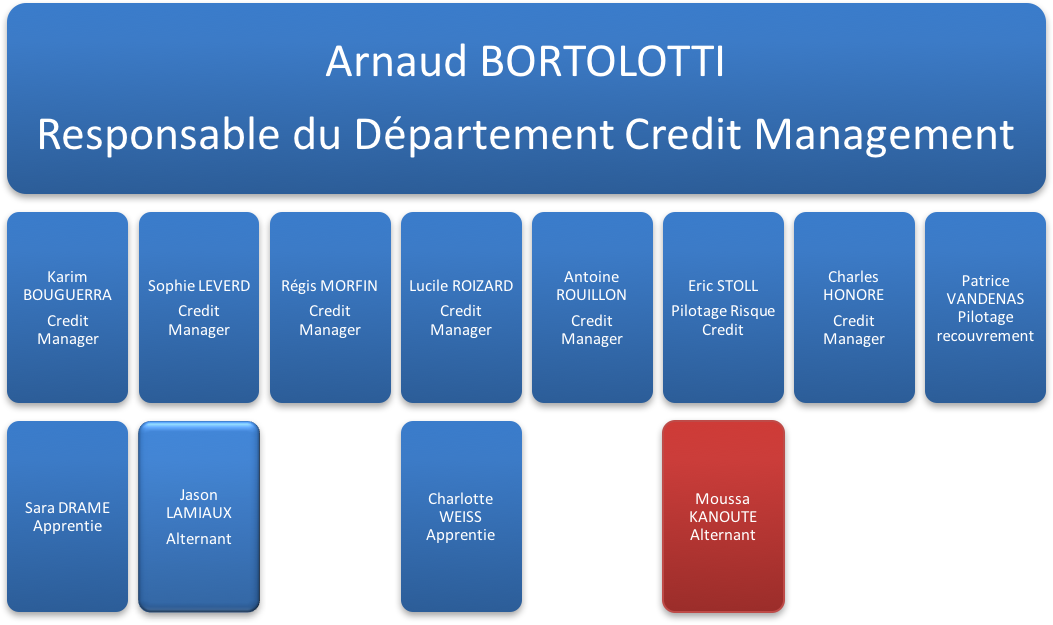
\includegraphics[scale=0.9]{cm_organigramme.png}
 \caption{Organigramme de la direction commerce EDF}
 \label{figure_cm}
\end{figure}
\subsection{Principe du Credit Management}
La crise financière de 2008 due à la titrisation des créances douteuses des emprunts immobiliers américains a mis à mal l’économie mondiale. Cette situation fait naître pour beaucoup de sociétés BtoB\footnote{BtoB: Business to Business= Marché des clients professionels} la nécessité vitale de se protéger des impayés et d’optimiser leur BFR.
\subparagraph{Principe de l'amont-aval:}
En amont, le Credit Manager a pour but de prévenir le risque de défaillance en mettant en place des garanties financières (Dépôt de garantie, Paiement d’avance, Modification du prix de vente, Limite de l’encours client,…). Le pilote risque de credit a pour but de suiveiller les ventes qui sont risqueés  en appliquant la polition de contre partie. \\\\
En aval, le Credit Manager doit veiller à ce que la situation des entreprises analysées ne se dégradent pas. Les garanties prises à un instant T peuvent ne plus correspondre au niveau de risque quelques mois plus tard. La veille permanente est un élément important dans la suivie du risque. 
Le recouvrement est un domaine important pour le Credit Manager. Dans le cadre de sa mission de gestion du BFR, il doit veiller à ce que les actions de recouvrement soient optimales afin de réduire l’impact des charges de créances irrécouvrables et participer à la mise en place des Best Practices
L’accompagnement des commerciaux dans vers une démarche de sélection des clients financièrement sains permet d’optimiser le rendement de l’entreprise. 
Permettre une prise de conscience des commerciaux sur le montant de marge à enregistrer pour compenser la perte engendrée par un client faisant défaut est un travail pédagogique indispensable. 

\section{Mes principales missions}

Dans cette section, je vais parler de mes principales missions au sein du service Credit Management. J'avais pour mission principale d'appuyer le pilote risque de credit. J'intervenais sur plusieurs sujets dont la production des activités de reportings, assurer le support et l'évolution  d'un outil de recouvrement et de relance des impayées au niveau national... 

\subsection{Implémentation d'un logiciel Business Intelligence Qlikview}
A mon arrivée dans l'épquipe, j'étais en charge de mettre en place des tableaux de bord permettant  à travers le logicel QlikView. L'objectif etait de migrer sur des outils plus efficaces en termine d'analyse et de prise de décisions. 
Dans un prémier temps, j'ai commencé à explorer les differentes fonctionnalités que propose Qlikiew et analyser la faisabilité des tableaux et des tâches quotidiennes. Ensuite, j'ai commencé à implémenter le logicel en mode itératif. Chaque intégration d'une nouvelle fonctionnalité était validée et testée par mes responsables. La figure suivante \ref{qlikview} montre le resultat une synthèse des différents que j'ai pu mettre en place. 
\begin{figure}[h]
 \centering
 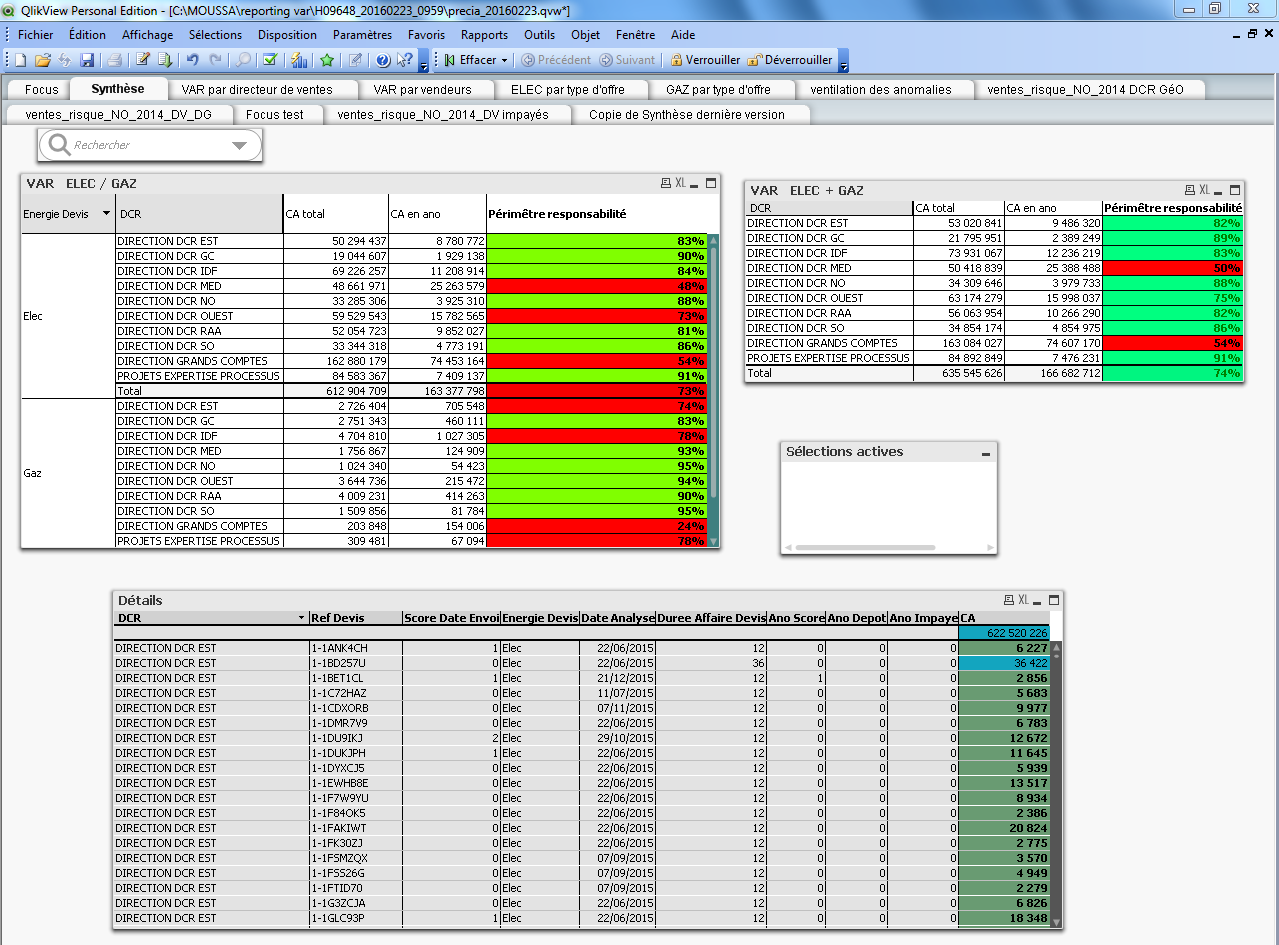
\includegraphics[scale=0.5]{qlik.PNG}
 \caption{Tableau de bord Qlikview}
 \label{qlikview}
\end{figure}

La figure ci-déssus montre trois tableaux de bords avec caracteristiques differents. L'avantages de Qlikview est qu'il permet d'avoir une synthèse des données de rapide dynamique et une exploration facile dans toutes les directions. Comme son nom l'indique, il suffit de cliquer sur une valeur pour visualiser les filtres s'appliquer automatiquement dans les autres tableaux. La figure \ref{qlikview_qlik} montre un exemple de sélection de données.

\begin{figure}[h]
 \centering
 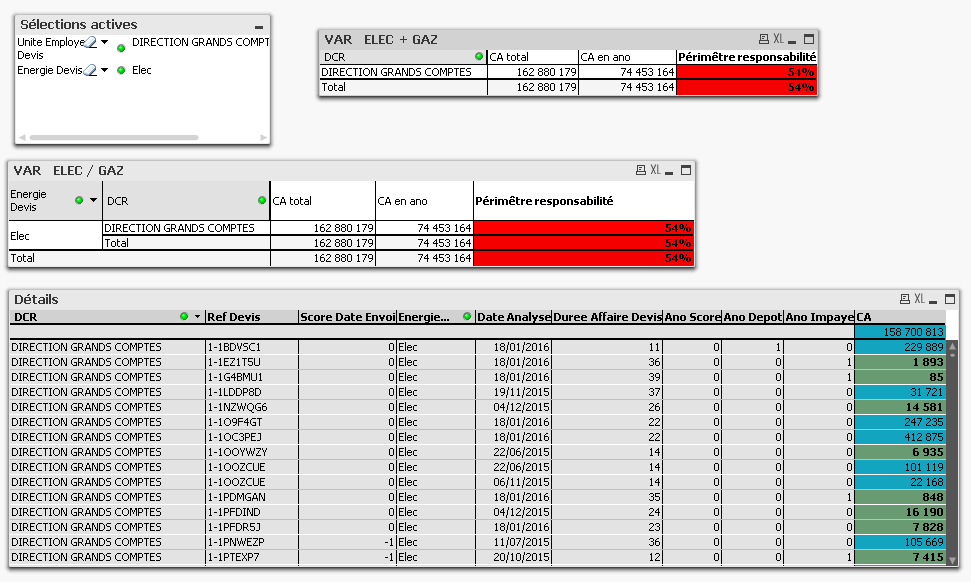
\includegraphics[scale=0.5]{exemple_qlikView.PNG}
 \caption{Exemple de parcours de données}
 \label{qlikview_qlik}
 
\end{figure}
\subsection{Réalisations de reporting à destination des à destination des plaques de recouvrement}
Outre la réalisation des tableaux de bord sur Qlikview, j'étais en charge de faire des reportings qui étaient destiner aux différentes plaques de recouvrement. Ce travail était réalisé en deux étapes: L'extraction et la consolidation de plusieurs sources de données d'une part et la constitution des portefeuilles clietns sous forme de fichiers.   

\subsubsection{Extraction et traitements des données}
La transformation des données avant exploitation est une étape importante et necésaire pour la bonne gouvernance des données. 
Avant tout je recupère les données à partir de differentes sources. Ces données proviennent d'autres entités du groupes. Dans la plupart des cas, je recupère une partie des données en planifiant des requêtes à travers des outils Business Objects internes au Groupe. Avant le stockage des différentes sources de données dans nos différents systèmes de gestion de base de données, il existe quelques étapes intermédiaires. 



\subsubsection{Production des reportings}


     
\begin{figure}[h]
 \centering
 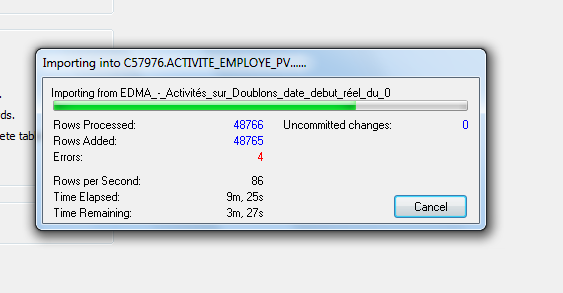
\includegraphics[scale=0.5]{import_fichier_toad.PNG}
 \caption{Modèle de tableau de bord Qlikview}
 \label{figure_cm}
\end{figure}
     \subsubsection{Application et suivi du risque de contre partie}
     
     
\subsection{Suivi d'un projet de restitution des données}
L'objectif de ce projet etait de definir et mettre à disposition des données brutes nécessaires à l’alimentation d'un prototype existant. Cela permettrait d’ores et déjà au service de disposer de toutes les données sur un même environnement. Ma mission sur principale dans ce projet était de verifier, comparer et valider des données mises à dispostion lorsque celles sont correspondent aux attentes. 

\subsection{Démarches}
\newpage
\section{Conclusion}
 
 

\newpage


 \newpage
 \bibliographystyle{plain}
\bibliography{bibliography.bib}
\end{document}